\section{Notes}


\textbf{Static variables:} Keep their values between unrelated calls to the function.

Global variables

Volatile

extern

\subsection{Floating Point Unit}
Floating point is a way to represent real numbers on computers.
IEEE floating point formats:

\begin{center}
	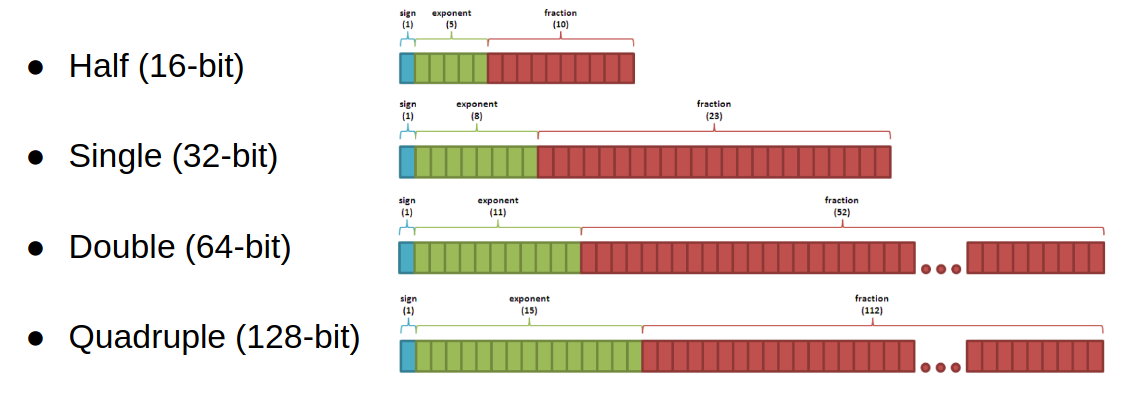
\includegraphics[width=\textwidth]{images/FPU.png}
\end{center}

The fraction part also known as the mantissa, describes
the significant digits of the number.
Where the exponent tells us where the decimal point is.



The FPU provides floating point computation functionality
that is compliant with the IEE 754 standard.
It enables conversion between fixed-point and floating-point data
formats, and floating-point constant instructions.

\subsection{Pointers}
Null pointer is a pointer used to initialize a pointer without
a memory address. It can be used as a function argument.

A void pointer is used to receive the address of a variable
of any data type.

\subsection{Strings}
In C a string is a line of characters pointed to by a pointer and
continuing until a $'\ 0'$ character is encountered.
The string might exist in memory of an array or as a constant.


\subsection{Queues}

A queue is an abstract data type that contains a collection of elements.
A queue object is an individual object in the task diagram.
As an object it has a name, number, id, key or handle and implement
a FIFO strategy. In addition to this it offers an API for
creating, inserting data, fetching data, show the state of the queue and
maybe read data without removing it from the queue (peek).


\begin{center}
	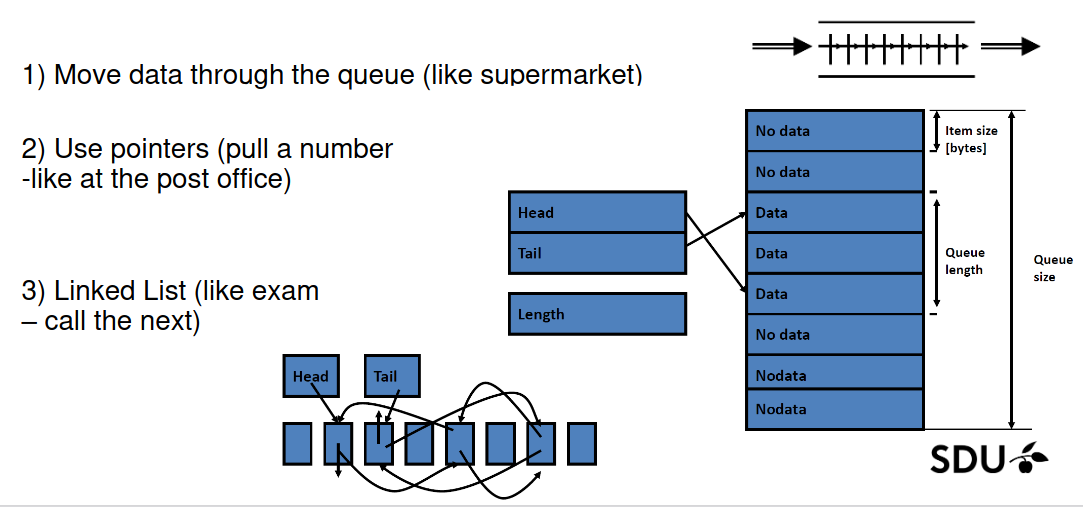
\includegraphics[width=\textwidth]{images/queue.png}
\end{center}

If a producer tries to write to a queue that is full, the producer
can throw away the data, do something else and try later,
overwrite old data or wait(block).



\subsection{Semaphores}

Real life: Visual signaling with arms and flags. A different example
can be parking access control.

There are two types of semaphores: binary and counting.

In software, a semaphore is a data structure for synchronization.
A semaphore is an integer varaible, but the only allowed operations
are increment and decrement. When a task decrements the
semaphore, if the results is neagtive,
the task blocks itself and cannot continue until
another task increments the semaphore.
When a task increments the semaphore, if there are other tasks waiting,
one of the waiting tasks gets unblocked.

Incrementing a semaphore is done using Signal() and decrementing
is called wait().

The reason for using semaphores is that it helps prevent bugs.
In addition to this the purposes of semaphores are to protect shared
variables, protect shared resources and critical sections.
Thus it helps with signaling (serialization)
by making sure that statements in different tasks/threads execute
in a specific order.

When using a semaphore for signaling you can have one task decrement the semaphore
and then a different task increment the semaphore.

Semaphore mutex is a type of semaphore that secures mutually exclusive
blocks to prevent concurrent access to the same resource.
A mutex is a binary semaphore that creates critical sections.

\begin{center}
	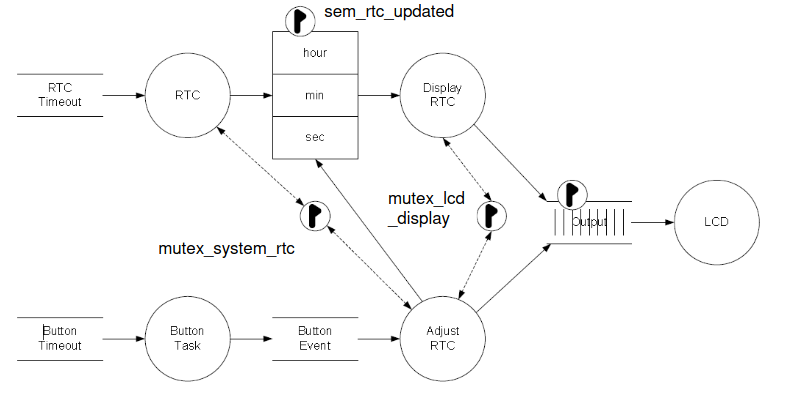
\includegraphics[width=\textwidth]{images/taskSemaphore.png}
\end{center}


\subsection{Debugging}
Simplest form of debugging is to toggle an LED pin to check execution.

Another form of debugging is to use an assert statement. This
is a macro that prints a message and halts the program if the
argument is false. The message contains line number and source file.

Otherwise you can use the serial port and write messages to a terminal.
However, this uses extra RAM and program memory for the printf routine.

PC simulation can be used but not for real-time testing.

ROM monitors are a cheap solution that uses RAM, ROM and execution time.
The good thing about a ROM monitor is that it is always available
but it can be problematic when debugging ISRs.

In Circuit Emulators are expensive but very powerful. This replaces the
microprocessor on the board. But they are problematic at high frequencies
because of the long wires.

In circuit debuggers or On-Chip Debuggers are the most common debuggers.
These consume no RAM or ROM and are always available. They are used
for debugging the hardware kernel.



\subsection{Build process}

A build process is hardware speficic. When using the TIVA controller
the compilation happens on the PC but for the TIVA controller, this
is called cross compilation. The compilation is handled by the IDE
(code composer studio)

\begin{center}
	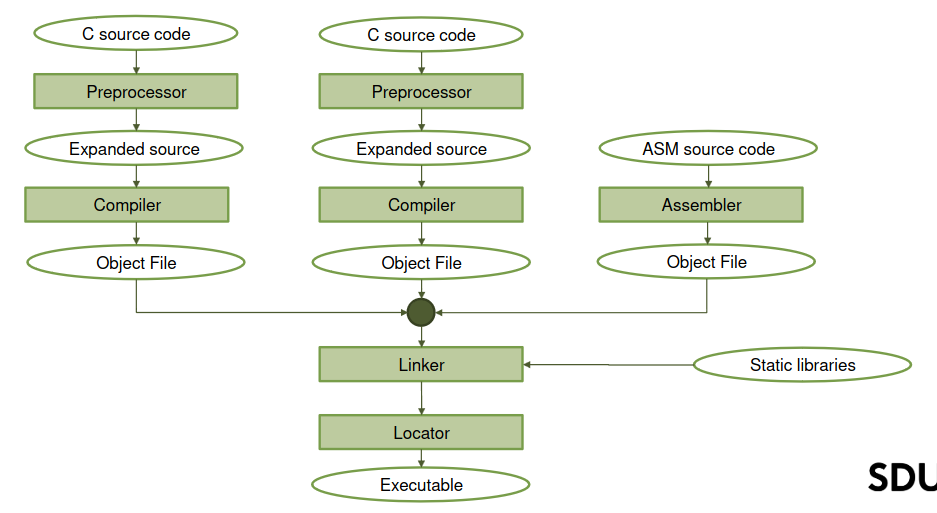
\includegraphics[width=\textwidth]{images/build.png}
\end{center}

The \textbf{preprocessor} handles preprocessor directives. This is what
starts with a \# in the code. This is for including libraries
and defines. In addition to this it removes comments and combines
split lines. The expanded code you get from copying header files
into the source code is then passed on to the compiler.

The \textbf{compiler} translates human readable code into machine code.
The output of a compiler is an object file, which is not executable.
Instead it is a binary file that contains instructions and data.

A \textbf{linker} linkes the object files together and resolves
any dependencies between them. It also links the libraries used
in the code. The output of the linker is relocatable and has no memory
addresses assigned to the code.
A relocatable program is a program that can be loaded into memory
at any address.

The \textbf{Locator} then transforms relocatable program into executable
binary image. Addresses are specified for each code line.


\subsection{Coding standards}
\begin{itemize}
	\item Think in abstraction levels
	\item limit module size
	\item Limit function size
	\item Comment your code
	\item Use proper indentation
	\item Use expressive file names
	\item Avoid: GOTO and CONTINUE
	\item Avoid code repetition
\end{itemize}

If a function contains more than 5 or 6 levels of indentation
or occupy more lines than presented on the screen, it should
be considered to break the function into sub functions.


RETURN should only be placed at the end of the function.
This can be ensured by using state variables instead of multiple
returns.

Avoid using abreveations in variable names, unless they are obvious.
Use underscores to seperate words.


\subsection{Logical vs bitwise}

Logical operators operate on bytes and words.
An expression is true if it not equal to zero. An expression is false
if it is equal to 0.

Bitwise operators perform logical functions by comparing bits one by one.



\subsection{Interrupts}
An interrupt is the automatic transfer of software execution in response to a hardware event that is asynchronous with the current software execution.

The hardware event is called a trigger. When this happens, an ISR is called.
This pauses the execution of the regular code, until the ISR returns or a
higher priority interrupt is triggered.


\subsection{Printf}

Printf in C is a function that prints formatted output.
Using printf one can format the string to contain embedded format tags
that are substituted with values.

An example of this is:
$printf("The value of x is \%d", x);$

\subsection{Deadlock}

A deadlock is when a process cannot proceed because
it needs to obtain a resource held by another process but
it itself is holding a resource that the other process needs.


\subsection{Assembler}
Low-level programming language.
Assembly code is very close to machine code instructions,
because of its direct mapping from assembler instructions
to procesor instructions.

Assembly language is a human readable programming language that
contains mnemonics of machine code (mov,ldr, ldi) etc.

Assember is a computer program that translates assembly source code
into machine language object code.

The reason as to why one would use assembly is because of its speed and size.
It can be used for strict timing requirements, where the execution time
is critical.


Assembly can be used inline in C code, like this:
$$ asm("MOV R0, \#0x01"); $$

A reccomended way to use assembly is to write the code in a seperate
file and then include it in the C code.



\subsection{Reentrancy}

A function is reentrant or pure if, while it is being executed,
can be called again by itself or by another function.
i.e. more than one instance of a function can run at the same time.

A function is reentrant if all variables are used atomic
or are allocated to the specific instance of the function (not static).

Atomic operations are operations that cannot be interrupted.
To ensure this, don't disable interrupts but
instead semaphores.


A function is \textbf{recursive} if it calls itself.
Thus, a recursive funciton must be reentrant.
